\documentclass[a4 paper]{article}

\usepackage[inner=2.0cm,outer=2.0cm,top=2.5cm,bottom=2.5cm]{geometry}
\usepackage{setspace}
\usepackage[rgb]{xcolor}
\usepackage{verbatim}
\usepackage{subcaption}
\usepackage{amsgen,amsmath,amstext,amsbsy,amsopn,tikz,amssymb,tkz-linknodes}
\usepackage{fancyhdr}
\usepackage[colorlinks=true, urlcolor=blue,  linkcolor=blue, citecolor=blue]{hyperref}
\usepackage[colorinlistoftodos]{todonotes}
\usepackage{rotating}
\usepackage{graphicx}
\usepackage{minted}

\setlength{\parindent}{0pt}

\allowdisplaybreaks
\DeclareMathOperator*{\argmin}{\arg\min} 
\DeclareMathOperator*{\argmax}{\arg\max} 

\hypersetup{%
pdfauthor={Vineeth S},%
pdftitle={Homework},%
pdfkeywords={Tikz,latex,bootstrap,uncertaintes},%
pdfcreator={PDFLaTeX},%
pdfproducer={PDFLaTeX},%
}

\usepackage{booktabs}
\newcommand{\ra}[1]{\renewcommand{\arraystretch}{#1}}

\newtheorem{thm}{Theorem}[section]
\newtheorem{prop}[thm]{Proposition}
\newtheorem{lem}[thm]{Lemma}
\newtheorem{cor}[thm]{Corollary}
\newtheorem{defn}[thm]{Definition}
\newtheorem{rem}[thm]{Remark}
\numberwithin{equation}{section}

\newcommand{\homework}[6]{
   \pagestyle{myheadings}
   \thispagestyle{plain}
   \newpage
   \setcounter{page}{1}
   \noindent
   \begin{center}
   \framebox{
      \vbox{\vspace{2mm}
    \hbox to 6.28in { {\bf E1 244:~Detection and Estimation Theory\hfill {\small (#2)}} }
       \vspace{6mm}
       \hbox to 6.28in { {\Large \hfill #1  \hfill} }
       \vspace{6mm}
       \hbox to 6.28in { {\it Instructor: {\rm #3} \hfill Name: {\rm #5}, SR No.: {\rm #6}} }
       %\hbox to 6.28in { {\it TA: #4  \hfill #6}}
      \vspace{2mm}}
   }
   \end{center}
   \markboth{#5 -- #1}{#5 -- #1}
   \vspace*{4mm}
}

\newcommand{\problem}[2]{~\\\fbox{\textbf{PART #1}}\hfill \newline\newline}
\newcommand{\subproblem}[2]{~\\\fbox{\text{#1}}\hfill \newline}
%\newcommand{\subproblem}[1]{~\newline\textbf{#1}}
\newcommand{\D}{\mathcal{D}}
\newcommand{\Hy}{\mathcal{H}}
\newcommand{\VS}{\textrm{VS}}
\newcommand{\solution}{~\newline\textbf{\textit{(Solution)}} }

\newcommand{\bbF}{\mathbb{F}}
\newcommand{\bbX}{\mathbb{X}}
\newcommand{\bI}{\mathbf{I}}
\newcommand{\bX}{\mathbf{X}}
\newcommand{\bY}{\mathbf{Y}}
\newcommand{\bepsilon}{\boldsymbol{\epsilon}}
\newcommand{\balpha}{\boldsymbol{\alpha}}
\newcommand{\bbeta}{\boldsymbol{\beta}}
\newcommand{\0}{\mathbf{0}}
\linespread{1.5}


\begin{document}

\setlength{\abovedisplayskip}{3pt}
\setlength{\belowdisplayskip}{3pt}

\homework{Assignment \#3}{Due: 22/06/20}{Sundeep Chepuri}{}{Vineeth S}{16543}

Consider a data symbol sequence $\mathbf{s} = [s[0], s[1], ..., s[N_{d} - 1]]^{T}$ of length $N_{d}$ , where the entries are QPSK with variance $\sigma_{s} = 1$, i.e., $s[k] \in \{\pm 1/ 2 \pm j/ 2\}$. According to the central limit theorem and assuming a sufficiently large IFFT, the OFDM symbol blocks $\mathbf{x}$ can be assumed to be zero-mean Gaussian with covariance matrix $E[\mathbf{x}\mathbf{x}^{H}] = \sigma_{s}^{2}\mathbf{I}_{(K+1)(N_{c} +N_{d})}$. $\mathbf{w}$ can be assumed to be a zero-mean complex Gaussian random process, where $E[\mathbf{w}\mathbf{w}^{H}] = \sigma_{w}^{2}\mathbf{I}_{(K+1)(N_c + N_d)}$. We wish to decide between the following two hypotheses:
\begin{align*}
	\mathcal{H}_{0} &: \mathbf{y} = \mathbf{w}	\\
	\mathcal{H}_{1} &: \mathbf{y} = \mathbf{x} + \mathbf{w}
\end{align*}

where $\mathbf{w} \sim \mathcal{CN}(0, \sigma_{n}^{2}\mathbf{I})$, and $\mathbf{w}$ is independent of $\mathbf{x}$.


\problem{A: Problem 1 Energy Detector}{}{}
\vspace{-2em}
\subproblem{Problem 1A Neyman-Pearson Detector}{}
\solution Consider the Neyman-Pearson likelihood ratio test. We decide on hypothesis $\mathcal{H}_{1}$ if
\begin{align*}
	L(y) = \frac{P(\mathbf{y}; \mathcal{H}_{1})}{P(\mathbf{y}; \mathcal{H}_{0})} > \gamma
\end{align*}

Let $N = (K + 1)(N_{d} + N_{c})$ for sake of simplicity.
\begin{align*}
	\mathcal{H}_{0}: y &\sim \mathcal{CN}(0, \sigma_{w}^{2}\mathbf{I}_{N})	\\
	\mathcal{H}_{1}: y &\sim \mathcal{CN}(0, (\sigma_{s}^{2} + \sigma_{w}^{2})\mathbf{I}_{N})	
\end{align*}


\begin{align*}
	\frac{\frac{1}{(2\pi)^{N/2}(\sigma_{s}^{2} + \sigma_{w}^{2})^{N/2}} exp \left(-\frac{1}{2(\sigma_{s}^{2} + \sigma_{w}^{2} )} \sum_{n=0}^{N-1} \vert y[n] \vert ^{2} \right)}{\frac{1}{(2\pi)^{N/2}(\sigma_{w}^{2})^{N/2}} exp \left(-\frac{1}{2\sigma_{w}^{2}} \sum_{n=0}^{N-1} \vert y[n] \vert ^{2} \right)} &> \gamma	\\
	\frac{(\sigma_{w}^{2})^{N/2}}{(\sigma_{s}^{2} + \sigma_{w}^{2})^{N/2}} exp \left(-\frac{1}{2} \sum_{n=0}^{N-1} \vert y[n] \vert ^{2} \left(\frac{1}{\sigma_{s}^{2} + \sigma_{w}^{2}} - \frac{1}{\sigma_{w}^{2}}\right) \right) &> \gamma \\
	\frac{1}{2} \sum_{n=0}^{N-1} \vert y[n] \vert ^{2} \left(\frac{\sigma_{s}^{2}}{(\sigma_{s}^{2} + \sigma_{w}^{2}) \sigma_{w}^{2}} \right) > \gamma^{,}	\\
	\sum_{n=0}^{N-1} \vert y[n] \vert ^{2} > \gamma^{,,}
\end{align*}

Hence, we have our test statistic $T(y)$ for NP detector as,
\begin{equation*}
	T(y) = 	\sum_{n=0}^{N-1} \vert y[n] \vert ^{2}
\end{equation*}


\newpage
We have our test statistic as sum of zero-mean Gaussian random variables. Hence the test statistic follows a $\chi_{N}^{2}$ distribution. 
\begin{align*}
	\mathcal{H}_{0} &: \frac{T(y)}{\sigma_{w}^{2}}	\sim \chi_{N}^{2}	\\
	\mathcal{H}_{1}	&: \frac{T(y)}{\sigma_{s}^{2} + \sigma_{w}^{2}}	\sim \chi_{N}^{2}
\end{align*}


For a specified $P_{FA}$ we can find the NP threshold as,
\begin{align*}
	P_{FA} &= P(T(y) > \gamma^{,,}; \mathcal{H}_{0})	\\
	P_{FA} &= Q_{\chi_{N}^{2}} \left( \frac{\gamma^{,,}}{\sigma_{w}^{2}}  \right)	\\
	\gamma^{,,} &= \sigma_{w}^{2} * Q_{\chi_{N}^{2}}^{-1} (P_{FA})
\end{align*}

And the theoretical detection probability $P_{D}$ as,
\begin{align*}
	P_{D} &= P(T(y) > \gamma^{,,}; \mathcal{H}_{1})	\\
		&= Q_{\chi_{N}^{2}} \left( \frac{\gamma^{,,}}{\sigma_{s}^{2} + \sigma_{w}^{2}}  \right)
\end{align*}

\subproblem{Problem 1B Bayes Detector}{}
\solution This part is related to the Problem 1C of PART B: Implementation. We are given that the primary user is mostly inactive with $P(\mathcal{H}_{1}) = 0.2$. Prior probabilities cannot be incorporated into Neyman-Pearson detector and hence we would be using Bayes detector for this case.

We decide on hypothesis $\mathcal{H}_{1}$ if
\begin{align*}
	L(y) = \frac{P(\mathbf{y}; \mathcal{H}_{1})}{P(\mathbf{y}; \mathcal{H}_{0})} > \frac{P(\mathcal{H}_{0})}{P(\mathcal{H}_{1})}
\end{align*}

Let $N = (K + 1)(N_{d} + N_{c})$ for sake of simplicity.
\begin{align*}
	\mathcal{H}_{0}: y &\sim \mathcal{CN}(0, \sigma_{w}^{2}\mathbf{I}_{N})	\\
	\mathcal{H}_{1}: y &\sim \mathcal{CN}(0, (\sigma_{s}^{2} + \sigma_{w}^{2})\mathbf{I}_{N})	
\end{align*}


\begin{align*}
	\frac{\frac{1}{(2\pi)^{N/2}(\sigma_{s}^{2} + \sigma_{w}^{2})^{N/2}} exp \left(-\frac{1}{2(\sigma_{s}^{2} + \sigma_{w}^{2} )} \sum_{n=0}^{N-1} \vert y[n] \vert ^{2} \right)}{\frac{1}{(2\pi)^{N/2}(\sigma_{w}^{2})^{N/2}} exp \left(-\frac{1}{2\sigma_{w}^{2}} \sum_{n=0}^{N-1} \vert y[n] \vert ^{2} \right)} &> \frac{P(\mathcal{H}_{0})}{P(\mathcal{H}_{1})}	\\
	\frac{(\sigma_{w}^{2})^{N/2}}{(\sigma_{s}^{2} + \sigma_{w}^{2})^{N/2}} exp \left(-\frac{1}{2} \sum_{n=0}^{N-1} \vert y[n] \vert ^{2} \left(\frac{1}{\sigma_{s}^{2} + \sigma_{w}^{2}} - \frac{1}{\sigma_{w}^{2}}\right) \right) &> \frac{P(\mathcal{H}_{0})}{P(\mathcal{H}_{1})} \\
	\frac{1}{2} \sum_{n=0}^{N-1} \vert y[n] \vert ^{2} \left(\frac{\sigma_{s}^{2}}{(\sigma_{s}^{2} + \sigma_{w}^{2}) \sigma_{w}^{2}} \right) &> ln \left( \frac{(\sigma_{s}^{2} + \sigma_{w}^{2})^{N/2}}{(\sigma_{w}^{2})^{N/2}}   	\frac{P(\mathcal{H}_{0})}{P(\mathcal{H}_{1})} \right)	\\   
\end{align*}

Hence, we have our test statistic $T(y)$ for Bayes detector as,
\begin{align*}
	T(y) = \sum_{n=0}^{N-1} \vert y[n] \vert ^{2} > 2 \left(\frac{(\sigma_{s}^{2} + \sigma_{w}^{2}) \sigma_{w}^{2}}{\sigma_{s}^{2}} \right) \left( \frac{N}{2} ln \left( \frac{\sigma_{s}^{2} + \sigma_{w}^{2}}{\sigma_{w}^{2}} \right) + ln P(\mathcal{H}_{0}) - ln P(\mathcal{H}_{1}) \right) 
\end{align*}


\newpage
\problem{A: Problem 2 Cyclostationary Detector}{}
\vspace{-2em}
\subproblem{Problem 2A Theory}{}
\solution Following the theory given in the problem statement, we have our test statistic $T(y)$ as,

\underline{\textbf{Under hypothesis $\mathcal{H}_{1}$}}	\\
\begin{align*}
	T(y) &= \sum_{n=0}^{N_{c}-1} \hat{R}[n])	\\
		&= \sum_{n=0}^{N_{c}-1} \frac{1}{K} \sum_{k=0}^{K-1} \hat{r}[n+kN, N_{d}]	\\
		&= \frac{1}{K} \sum_{n=0}^{N_{c}-1} \sum_{k=0}^{K-1} y[n+kN] y^{*} [n+kN+N_{d}]	\\
\end{align*}

For $n=0, .., N_{c} -1$, let
\begin{align*}
	y[n+kN] = x + w_{1}	\\
	y[n+kN+N_{d}] = x + w_{2}
\end{align*}

Let $z =  y[n+kN] y^{*} [n+kN+N_{d}]$.

We have,
\begin{align*}
	E[z] &= E[(x + w_{1})(x + w_{2})^{*}]	\\
		&= E[\vert x \vert ^{2} + xw_{2}^{*} + x^{*}w_{1} + w_{1}w_{2}^{*}]	\\
		&= E[\vert x \vert ^{2}]	\\
		&= \sigma_{s}^{2}	\\
		&= 1
\end{align*}

\begin{align*}
	E[T(y)] &= \frac{1}{K} \sum_{n=0}^{N_{c}-1} \sum_{k=0}^{K-1} E[y[n+kN] y^{*} [n+kN+N_{d}]]	\\
		&= \frac{1}{K} N_{c} K	\\
		&= N_{c}
\end{align*}
\begin{align*}
	T^{2}(y) &= \frac{1}{K^{2}} \sum_{n_{1}=0}^{N_{c}-1} \sum_{k_{1}=0}^{K-1} \sum_{n_{2}=0}^{N_{c}-1} \sum_{k_{2}=0}^{K-1} y[n_{1}+k_{1}N] y^{*} [n_{1}+k_{1}N+N_{d}] y[n_{2}+k_{2}N] y^{*} [n_{2}+k_{2}N+N_{d}]
\end{align*}


For $n=0, .., N_{c} -1$, let
\begin{align*}
	y[n_{1} + k_{1}N] &= x_{1} + w_{11}			&y[n_{2}+k_{2}N] = x_{2} + w_{21}		\\
	y[n_{1} + k_{1}N+N_{d}] &= x_{1} + w_{12}		&y[n_{2}+k_{2}N+N_{d}] = x_{2} + w_{22}
\end{align*}

Let $z = y[n_{1}+k_{1}N] y^{*} [n_{1}+k_{1}N+N_{d}] y[n_{2}+k_{2}N] y^{*} [n_{2}+k_{2}N+N_{d}]$


For $n_{1} \neq n_{2}$ or $k_{1} \neq k_{2}$, $x_{1}$ and $x_{2}$ are independent,
\begin{align*}
	E[z] &= E[(x_{1} + w_{11}) (x_{1} + w_{12})^{*} (x_{2} + w_{21}) (x_{2} + w_{22})^{*}]	\\
		&= E[(x_{1} + w_{11}) (x_{1} + w_{12})^{*}] E[(x_{2} + w_{21}) (x_{2} + w_{22})^{*}]	\\
		&= \sigma_{s}^{4}	\\
		&= 1
\end{align*}

For $n_{1} = n_{2}$ and $k_{1} = k_{2}$,
\begin{align*}
	E[z] &= E[(x_{1} + w_{11}) (x_{1} + w_{12})^{*} (x_{1} + w_{11}) (x_{1} + w_{12})^{*}]	\\
		&= E[(\vert x_{1} \vert ^{2} + x_{1}w_{12}^{*} + x_{1}^{*}w_{11} + w_{11}w_{12}^{*})^{2}]	\\
		&= E[\vert x_{1} \vert ^{4}]	\\
		&= 2\sigma_{s}^{4}	\\
		&= 2
\end{align*}

where $ \vert x_{1} \vert = \sqrt{Re(x_{1})^{2} + Im(x_{1})^{2}}$ and hence $\vert x_{1} \vert$ follows Rayleigh distribution. Using the equation for fourth moment of Rayleigh random variable, we have $E[\vert x_{1} \vert ^{4}] = 2\sigma_{s}^{4}$. Also, from complex Gaussian distribution properties we have, $E[w_{ij}] = 0$ and $E[w_{ij}^{2}] = 0$. Hence we have,
\begin{align*}
	E[T^{2}(y)] &= \frac{1}{K^{2}} \sum_{n_{1}=0}^{N_{c}-1} \sum_{k_{1}=0}^{K-1} \sum_{n_{2}=0}^{N_{c}-1} \sum_{k_{2}=0}^{K-1} E[(y[n_{1}+k_{1}N] y^{*} [n_{1}+k_{1}N+N_{d}] y[n_{2}+k_{2}N] y^{*} [n_{2}+k_{2}N+N_{d}]]	\\
		&= \frac{1}{K^{2}} [2N_{c} K + N_{c}^{2}K^{2} - N_{c}K]	\\
		&= N_{c}^{2} + \frac{N_{c}}{K}
\end{align*}

Similarly,
\begin{align*}
	\lvert T(y) \rvert^{2} &= \frac{1}{K^{2}} \sum_{n_{1}=0}^{N_{c}-1} \sum_{k_{1}=0}^{K-1} \sum_{n_{2}=0}^{N_{c}-1} \sum_{k_{2}=0}^{K-1} y[n_{1}+k_{1}N] y^{*} [n_{1}+k_{1}N+N_{d}] y^{*}[n_{2}+k_{2}N] y [n_{2}+k_{2}N+N_{d}]
\end{align*}

Let $z = y[n_{1}+k_{1}N] y^{*} [n_{1}+k_{1}N+N_{d}] y^{*}[n_{2}+k_{2}N] y [n_{2}+k_{2}N+N_{d}]$


For $n_{1} \neq n_{2}$ or $k_{1} \neq k_{2}$, $x_{1}$ and $x_{2}$ are independent,
\begin{align*}
	E[z] &= E[(x_{1} + w_{11}) (x_{1} + w_{12})^{*} (x_{2} + w_{21})^{*} (x_{2} + w_{22})]	\\
	&= E[(x_{1} + w_{11}) (x_{1} + w_{12})^{*}] E[(x_{2} + w_{21})^{*} (x_{2} + w_{22})]	\\
	&= \sigma_{s}^{4}	\\
	&= 1
\end{align*}


For $n_{1} = n_{2}$ and $k_{1} = k_{2}$,
\begin{align*}
	E[z] &= E[(x_{1} + w_{11}) (x_{1} + w_{12})^{*} (x_{1} + w_{11})^{*} (x_{1} + w_{12})]	\\
	&= E[(\vert x_{1} \vert ^{2} + x_{1}w_{12}^{*} + x_{1}^{*}w_{11} + w_{11}w_{12}^{*}) (\vert x_{1} \vert ^{2} + x_{1}^{*}w_{12} + x_{1}w_{11}^{*} + w_{11}^{*}w_{12}]	\\
		&= E[\lvert x_{1} \rvert^{4} + \lvert x_{1} \rvert^{2} \lvert w_{12} \rvert^{2} + \lvert x_{1} \rvert^{2} \lvert w_{11} \rvert^{2} + \lvert w_{11} \rvert^{2} \lvert w_{12} \rvert^{2}]	\\
		&= 2\sigma_{s}^{4} + 2\sigma_{s}^{2}\sigma_{w}^{2} + \sigma_{w}^{4}	\\
		&= 2 + 2\sigma_{w}^{2} + \sigma_{w}^{4}
\end{align*}

Hence we have,
\begin{align*}
	E[\lvert T(y) \rvert^{2}] &= \frac{1}{K^{2}} \sum_{n_{1}=0}^{N_{c}-1} \sum_{k_{1}=0}^{K-1} \sum_{n_{2}=0}^{N_{c}-1} \sum_{k_{2}=0}^{K-1} E[(y[n_{1}+k_{1}N] y^{*} [n_{1}+k_{1}N+N_{d}] y^{*} [n_{2}+k_{2}N] y [n_{2}+k_{2}N+N_{d}]]	\\
	&= \frac{1}{K^{2}} [N_{c} K (2 + 2\sigma_{w}^{2} + \sigma_{w}^{4}) + N_{c}^{2}K^{2} - N_{c}K]	\\
	&= N_{c}^{2} + \frac{N_{c}}{K} (1 + 2\sigma_{w}^{2} + \sigma_{w}^{4})
\end{align*}

Summarizing all data we have,
\begin{align*}
	E[T] &= N_{c} \\
	E[T^{2}(y)] &= N_{c}^{2} + \frac{N_{c}}{K}	&= E[\bar{T}^{2} + j2\bar{T}\tilde{T} -\tilde{T}^{2}]	\\
	E[\lvert T(y) \rvert^{2}] &= N_{c}^{2} + \frac{N_{c}}{K} (1 + 2\sigma_{w}^{2} + \sigma_{w}^{4})	&= E[\bar{T}^{2} -\tilde{T}^{2}]
\end{align*}

Solving we have,
\begin{align*}
	E[\bar{T}] &= N_{c}  \\
	E[\tilde{T}] &= 0 	\\
	E[\bar{T}\tilde{T}] &= 0	\\
	E[\bar{T}^{2}] &= N_{c}^{2} + \frac{N_{c}}{K} (1 + \sigma_{w}^{2} + \frac{\sigma_{w}^{4}}{2})	\\
	E[\tilde{T}^{2}] &= \frac{N_{c}}{K} (\sigma_{w}^{2} + \frac{\sigma_{w}^{4}}{2})	\\
\end{align*}

Finally we have,
\begin{align*}
	E[\bar{T}] &= N_{c}  \\
	Var(\bar{T}) &= \frac{N_{c}}{K} (1 + \sigma_{w}^{2} + \frac{\sigma_{w}^{4}}{2})	\\
	E[\tilde{T}] &= 0 	\\
	Var(\tilde{T}) &= \frac{N_{c}}{K} (\sigma_{w}^{2} + \frac{\sigma_{w}^{4}}{2})	\\
	Cov(\bar{T}\tilde{T}) &= 0
\end{align*}

\underline{\textbf{Under hypothesis $\mathcal{H}_{0}$}}	\
\begin{align*}
	T(y) &= \sum_{n=0}^{N_{c}-1} \hat{R}[n])	\\
	&= \sum_{n=0}^{N_{c}-1} \frac{1}{K} \sum_{k=0}^{K-1} \hat{r}[n+kN, N_{d}]	\\
	&= \frac{1}{K} \sum_{n=0}^{N_{c}-1} \sum_{k=0}^{K-1} y[n+kN] y^{*} [n+kN+N_{d}]	\\
\end{align*}

For $n=0, .., N_{c} -1$, let
\begin{align*}
	y[n+kN] = w_{1}	\\
	y[n+kN+N_{d}] = w_{2}
\end{align*}

Let $z =  y[n+kN] y^{*} [n+kN+N_{d}]$.

We have,
\begin{align*}
	E[z] &= E[w_{1}w_{2}^{*}]	\\
	&= 0
\end{align*}

\begin{align*}
	E[T(y)] &= \frac{1}{K} \sum_{n=0}^{N_{c}-1} \sum_{k=0}^{K-1} E[y[n+kN] y^{*} [n+kN+N_{d}]]	\\
	&= 0
\end{align*}
\begin{align*}
	T^{2}(y) &= \frac{1}{K^{2}} \sum_{n_{1}=0}^{N_{c}-1} \sum_{k_{1}=0}^{K-1} \sum_{n_{2}=0}^{N_{c}-1} \sum_{k_{2}=0}^{K-1} y[n_{1}+k_{1}N] y^{*} [n_{1}+k_{1}N+N_{d}] y[n_{2}+k_{2}N] y^{*} [n_{2}+k_{2}N+N_{d}]
\end{align*}


For $n=0, .., N_{c} -1$, let
\begin{align*}
	y[n_{1} + k_{1}N] &= w_{11}			&y[n_{2}+k_{2}N] = w_{21}		\\
	y[n_{1} + k_{1}N+N_{d}] &= w_{12}		&y[n_{2}+k_{2}N+N_{d}] = w_{22}
\end{align*}

Let $z = y[n_{1}+k_{1}N] y^{*} [n_{1}+k_{1}N+N_{d}] y[n_{2}+k_{2}N] y^{*} [n_{2}+k_{2}N+N_{d}]$


For $n_{1} \neq n_{2}$ or $k_{1} \neq k_{2}$, $x_{1}$ and $x_{2}$ are independent,
\begin{align*}
	E[z] &= E[w_{11} w_{12}^{*} w_{21} w_{22}^{*}]	\\
		&= E[w_{11}] E[w_{12}^{*}] E[w_{21}] E[w_{22}^{*}]	\\
		&= 0
\end{align*}

For $n_{1} = n_{2}$ and $k_{1} = k_{2}$,
\begin{align*}
	E[z] &= E[w_{11} w_{12}^{*} w_{11} w_{12}^{*}]	\\
		&=  E[\lvert w_{11} \rvert^{2} \lvert w_{12} \rvert^{2}]	\\
		&= \sigma_{w}^{4}
\end{align*}
\begin{align*}
	E[T^{2}(y)] &= \frac{1}{K^{2}} \sum_{n_{1}=0}^{N_{c}-1} \sum_{k_{1}=0}^{K-1} \sum_{n_{2}=0}^{N_{c}-1} \sum_{k_{2}=0}^{K-1} E[(y[n_{1}+k_{1}N] y^{*} [n_{1}+k_{1}N+N_{d}] y[n_{2}+k_{2}N] y^{*} [n_{2}+k_{2}N+N_{d}]]	\\
		&= \frac{1}{K^{2}} [N_{c} K \sigma_{w}^{4}]	\\
		&= \frac{N_{c}}{K} \sigma_{w}^{4}
\end{align*}


Similarly,
\begin{align*}
	\lvert T(y) \rvert^{2} &= \frac{1}{K^{2}} \sum_{n_{1}=0}^{N_{c}-1} \sum_{k_{1}=0}^{K-1} \sum_{n_{2}=0}^{N_{c}-1} \sum_{k_{2}=0}^{K-1} y[n_{1}+k_{1}N] y^{*} [n_{1}+k_{1}N+N_{d}] y^{*}[n_{2}+k_{2}N] y [n_{2}+k_{2}N+N_{d}]
\end{align*}

Let $z = y[n_{1}+k_{1}N] y^{*} [n_{1}+k_{1}N+N_{d}] y^{*}[n_{2}+k_{2}N] y [n_{2}+k_{2}N+N_{d}]$

For $n_{1} \neq n_{2}$ or $k_{1} \neq k_{2}$, $x_{1}$ and $x_{2}$ are independent,
\begin{align*}
	E[z] &= E[w_{11} w_{12}^{*} w_{21}^{*} w_{22}]	\\
		&= E[w_{11}] E[w_{12}^{*}] E[w_{21}^{*}] E[w_{22}]	\\
		&= 0
\end{align*}


For $n_{1} = n_{2}$ and $k_{1} = k_{2}$,
\begin{align*}
	E[z] &= E[w_{11} w_{12}^{*} w_{11}^{*} w_{12}]	\\
		&= E[\lvert w_{11} \rvert^{2} \lvert w_{12} \rvert^{2}]	\\
		&= \sigma_{w}^{4}
\end{align*}

Hence we have,
\begin{align*}
	E[\lvert T(y) \rvert^{2}] &= \frac{1}{K^{2}} \sum_{n_{1}=0}^{N_{c}-1} \sum_{k_{1}=0}^{K-1} \sum_{n_{2}=0}^{N_{c}-1} \sum_{k_{2}=0}^{K-1} E[(y[n_{1}+k_{1}N] y^{*} [n_{1}+k_{1}N+N_{d}] y^{*} [n_{2}+k_{2}N] y [n_{2}+k_{2}N+N_{d}]]	\\
		&= \frac{1}{K^{2}} [N_{c} K \sigma_{w}^{4}]	\\
		&= \frac{1}{K} N_{c} \sigma_{w}^{4}
\end{align*}

Summarizing all data we have,
\begin{align*}
	E[T] &= 0 \\
	E[T^{2}(y)] &= \frac{1}{K} N_{c} \sigma_{w}^{4}	&= E[\bar{T}^{2} + j2\bar{T}\tilde{T} -\tilde{T}^{2}]	\\
	E[\lvert T(y) \rvert^{2}] &= \frac{1}{K} N_{c} \sigma_{w}^{4}	&= E[\bar{T}^{2} -\tilde{T}^{2}]
\end{align*}

Solving we have,
\begin{align*}
	E[\bar{T}] &= 0  \\
	E[\tilde{T}] &= 0 	\\
	E[\bar{T}\tilde{T}] &= 0	\\
	E[\bar{T}^{2}] &= \frac{N_{c}}{2K} \sigma_{w}^{4}	\\
	E[\tilde{T}^{2}] &= \frac{N_{c}}{2K} \sigma_{w}^{4}	\\
\end{align*}

Finally we have,
\begin{align*}
	E[\bar{T}] &= 0 \\
	Var(\bar{T}) &= \frac{N_{c}}{2K} \sigma_{w}^{4}		\\
	E[\tilde{T}] &= 0 	\\
	Var(\tilde{T}) &= \frac{N_{c}}{2K} \sigma_{w}^{4}		\\
	Cov(\bar{T}\tilde{T}) &= 0
\end{align*}


\newpage
\subproblem{Problem 2B Neyman-Pearson Detector}{}
We decide on $\mathcal{H}_{1}$ if $\lvert T(y) \rvert > \gamma$. Or equivalently if $\lvert T(y) \rvert^{2} > \gamma^{2}$.


For a specified $P_{FA}$ we can find the NP threshold as,
\begin{align*}
	P_{FA} &= P(\lvert T(y) \rvert > \gamma; \mathcal{H}_{0})	\\
	P_{FA} &= P(\lvert T(y) \rvert^{2} > \gamma^{2}; \mathcal{H}_{0})	\\
	P_{FA} &= P(\bar{T}^{2}(y) + \tilde{T}^{2}(y) > \gamma^{2}; \mathcal{H}_{0})	\\		
	P_{FA} &= Q_{\chi_{2}^{2}} \left( \frac{\gamma^{2}}{\frac{N_{c}}{2K}\sigma_{w}^{4}}  \right)	\\
	\gamma^{2} &= \frac{N_{c}}{2K}\sigma_{w}^{4} * Q_{\chi_{2}^{2}}^{-1} (P_{FA})
\end{align*}


\newpage
\problem{B: Energy Detector}{}
\vspace{-2em}
\subproblem{Subpart A}{}
\vspace{-2em}
\begin{figure}[h]
	\centering
	\begin{subfigure}{.5\textwidth}
		%\centering
		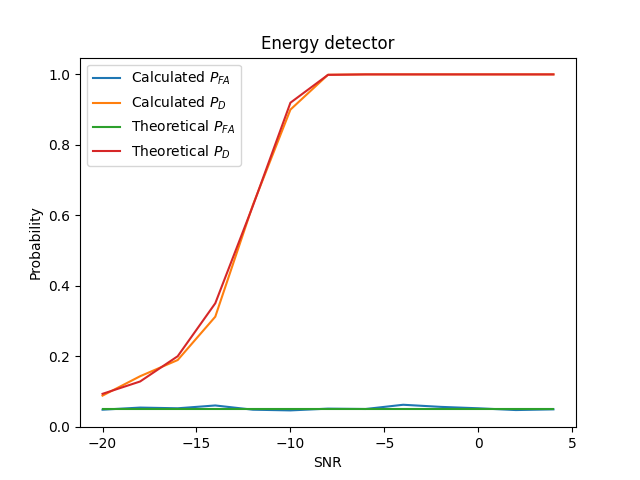
\includegraphics[width=1\linewidth]{../results/energy_detector_a.png}
		\caption{For 1000 records}
		\label{fig:energy_a1}
	\end{subfigure}%
	\begin{subfigure}{.5\textwidth}
		%\centering
		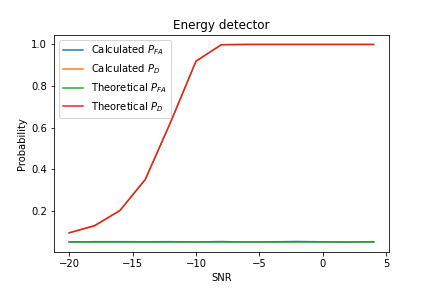
\includegraphics[width=1.15\linewidth]{../results/energy_detector_a_ideal.png}
		\caption{For 100000 records}
		\label{fig:energy_a2}
	\end{subfigure}
	\caption{Probability vs SNR}
	\label{fig:energy_a}
\end{figure}

From the plot Figure(\ref{fig:energy_a}), we can easily observe that the theoretical $P_{d}$ and calculated $P_{d}$ increases with the SNR value. We can also verify that $P_{FA}$ is under 0.05. Figure(\ref{fig:energy_a1}) represents the detector performance with 1000 statistics and Figure(\ref{fig:energy_a2}) represents the detector performance with 100000 statistics. We can see that with increased number of test statistics, we get the ideal detector performance. 


\subproblem{Subpart B}{}
\vspace{-2em}
\begin{figure}[h]
	\centering
	\begin{subfigure}{.5\textwidth}
		%\centering
		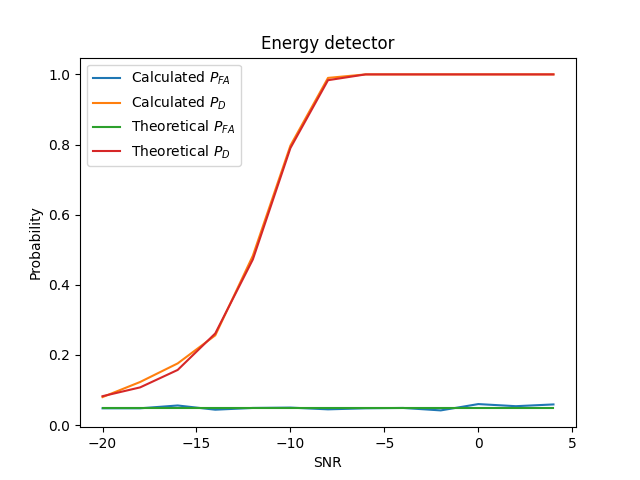
\includegraphics[width=1\linewidth]{../results/energy_detector_b.png}
		\caption{For 1000 records}
		\label{fig:energy_b1}
	\end{subfigure}%
	\begin{subfigure}{.5\textwidth}
		%\centering
		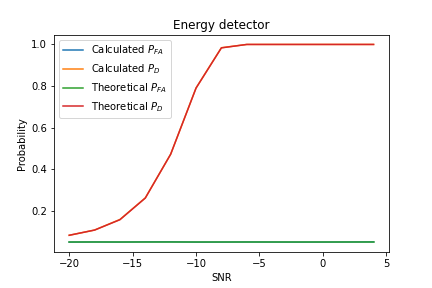
\includegraphics[width=1.15\linewidth]{../results/energy_detector_b_ideal.png}
		\caption{For 100000 records}
		\label{fig:energy_b2}
	\end{subfigure}
	\caption{Probability vs SNR}
	\label{fig:energy_b}
\end{figure}


From the plot Figure(\ref{fig:energy_b}), we can observe a clear drop in theoretical $P_{d}$ and calculated $P_{d}$ compared to the previous case when we have noisy estimates.. However the performance drop is negligible for higher values of SNR --- owing to the smaller noise component. Figure(\ref{fig:energy_b1}) represents the detector performance with 1000 statistics and Figure(\ref{fig:energy_b2}) represents the detector performance with 100000 statistics. We can see that with increased number of test statistics, we get the ideal detector performance. 


\subproblem{Subpart C}{}
\vspace{-2em}
\begin{figure}[h]
	\centering
	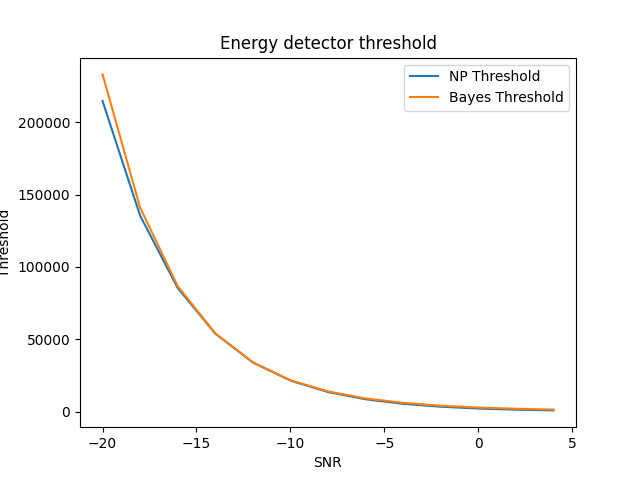
\includegraphics[width=0.75\linewidth]{../results/energy_detector_c.png}
	\caption{Threshold}
	\label{fig:energy_c}
\end{figure}

Figure(\ref{fig:energy_c}) shows the threshold variation with respect to SNR for Neyman-Pearson detector and Bayes detector. We can observe that the NP threshold is slightly lesser than Bayes threshold for lower values of SNR. As the value of SNR increases, the noise component in the observed signal decreases, and hence the variance of observed signal decreases. As a result, the detector threshold decreases.



\newpage

\problem{B: Cyclostationary Detector}{}
\vspace{-2em}
\subproblem{Subpart A}{}
\vspace{-1em}


From the plots Figure(\ref{fig:cyclo_a}) and Figure(\ref{fig:cyclo_ai}), we can verify that the means and variances match with the same of that of the complex Gaussian distribution we derived. Figure(\ref{fig:cyclo_a}) represents the detector performance with 1000 statistics and Figure(\ref{fig:cyclo_ai}) represents the detector performance with 100000 statistics. We can see that with increased number of test statistics, we get the ideal probability distribution. 

\begin{figure}[h]
	\centering
	\begin{subfigure}{.5\textwidth}
		%\centering
		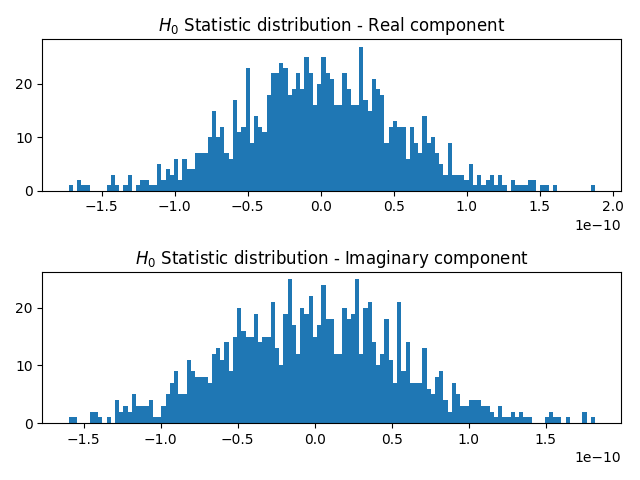
\includegraphics[width=1\linewidth]{../results/cyclostationary_detector_a_H0.png}
		\caption{Hypothesis $\mathcal{H}_{0}$}
		\label{fig:cyclo_a1}
	\end{subfigure}%
	\begin{subfigure}{.5\textwidth}
		%\centering
		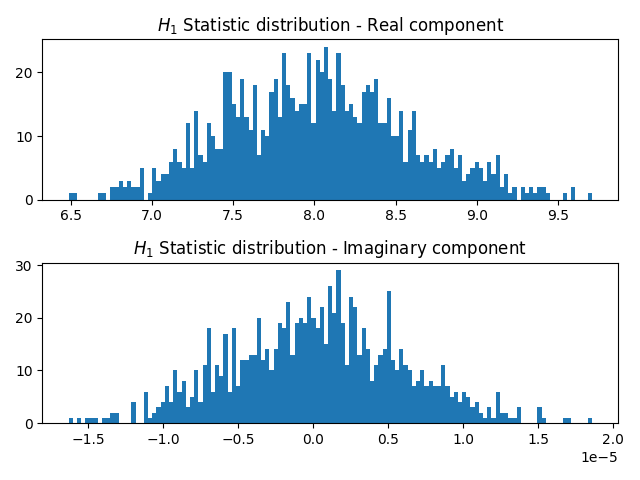
\includegraphics[width=1\linewidth]{../results/cyclostationary_detector_a_H1.png}
		\caption{Hypothesis $\mathcal{H}_{1}$}
		\label{fig:cyclo_a2}
	\end{subfigure}
	\caption{Distribution for 1000 statistics}
	\label{fig:cyclo_a}
\end{figure}


\vspace{-1em}
\begin{figure}[h]
	\centering
	\begin{subfigure}{.5\textwidth}
		%\centering
		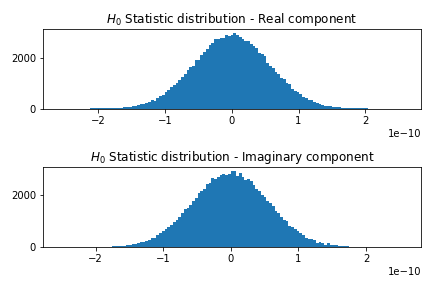
\includegraphics[width=1\linewidth]{../results/cyclostationary_detector_a_H0_ideal.png}
		\caption{Hypothesis $\mathcal{H}_{0}$}
		\label{fig:cyclo_ai1}
	\end{subfigure}%
	\begin{subfigure}{.5\textwidth}
		%\centering
		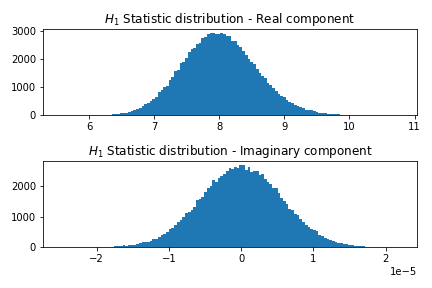
\includegraphics[width=1\linewidth]{../results/cyclostationary_detector_a_H1_ideal.png}
		\caption{Hypothesis $\mathcal{H}_{1}$}
		\label{fig:cyclo_ai2}
	\end{subfigure}
	\caption{Distribution for 100000 statistics}
	\label{fig:cyclo_ai}
\end{figure}


\vspace{-1em}
\subproblem{Subpart B}{}
\vspace{-1em}

From the plot Figure(\ref{fig:cyclo_b}), we can easily observe that the calculated $P_{d}$ increases with the SNR value. We can also verify that $P_{FA}$ is under 0.05. Figure(\ref{fig:cyclo_b1}) represents the detector performance with 1000 statistics and Figure(\ref{fig:cyclo_b2}) represents the detector performance with 100000 statistics. We can see that with increased number of test statistics, we get the ideal detector performance. 

Comparing energy detector performance with cyclostationary detector performance, we can observe that energy detector gives much higher values of $P_{D}$ for the same SNR value. Also, energy detector achieves higher values of $P_{D}$ for lower SNR value. For example, energy detector achieves $P_{D}$ values close to 1 around -10dB whereas cyclostationary detector achieves it around -5dB. For lower values of SNR, energy detector clearly outperforms cyclostationary detector by a huge margin.

\begin{figure}[h]
	\centering
	\begin{subfigure}{.5\textwidth}
		%\centering
		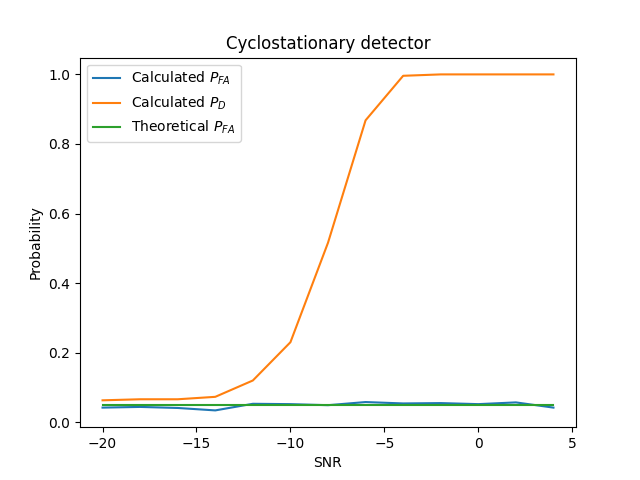
\includegraphics[width=1\linewidth]{../results/cyclostationary_detector_b.png}
		\caption{For 1000 records}
		\label{fig:cyclo_b1}
	\end{subfigure}%
	\begin{subfigure}{.5\textwidth}
		%\centering
		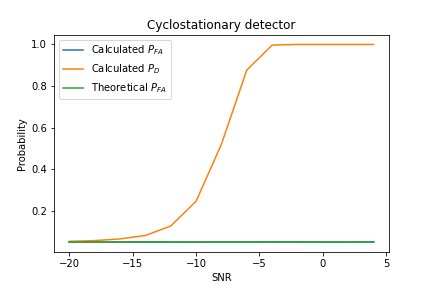
\includegraphics[width=1.15\linewidth]{../results/cyclostationary_detector_b_ideal.png}
		\caption{For 100000 records}
		\label{fig:cyclo_b2}
	\end{subfigure}
	\caption{Probability vs SNR}
	\label{fig:cyclo_b}
\end{figure}


\vspace{-2em}
\subproblem{Subpart C}{}
\vspace{-1em}

From the plot Figure(\ref{fig:cyclo_c}), we can observe a clear drop in calculated $P_{d}$ compared to the previous case. However the performance drop is negligible for higher values of SNR --- owing to the smaller noise component. We can also observe that the drop in performance for cyclostationary detector is lesser compared to same case with energy detector and hence it is less prone to noisy estimates. Figure(\ref{fig:cyclo_c1}) represents the detector performance with 1000 statistics and Figure(\ref{fig:cyclo_c2}) represents the detector performance with 100000 statistics. We can see that with increased number of test statistics, we get the ideal detector performance. 
\begin{figure}[h]
	\centering
	\begin{subfigure}{.5\textwidth}
		%\centering
		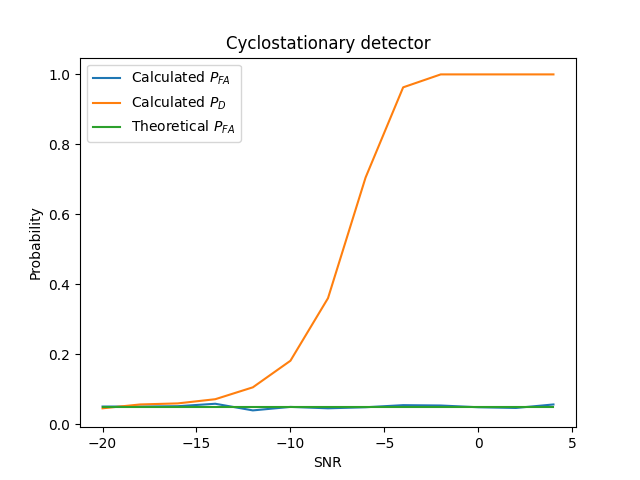
\includegraphics[width=1\linewidth]{../results/cyclostationary_detector_c.png}
		\caption{For 1000 records}
		\label{fig:cyclo_c1}
	\end{subfigure}%
	\begin{subfigure}{.5\textwidth}
		%\centering
		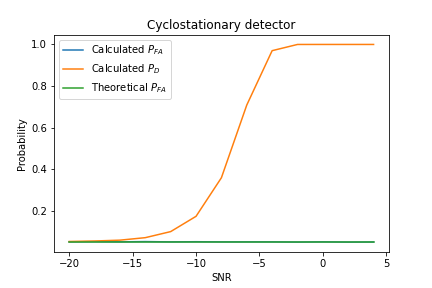
\includegraphics[width=1.15\linewidth]{../results/cyclostationary_detector_c_ideal.png}
		\caption{For 100000 records}
		\label{fig:cyclo_c2}
	\end{subfigure}
	\caption{Probability vs SNR}
	\label{fig:cyclo_c}
\end{figure}



\newpage
\problem{C: Appendices (Python codes)}{}
\solution The entire program is written in six python files. The codes are provided below and are also available at \url{https://github.com/vineeths96/Spectrum-sensing-for-cognitive-radio} GitHub repository. (Repository access is private as of now. Access can me made available, if necessary).

\subproblem{Problem 1A}{}
\inputminted[frame=lines, framesep=2mm, baselinestretch=1.2, fontsize=\footnotesize, linenos]{python3}{'../energy_detector/energy_detector_a.py'}

\subproblem{Problem 1B}{}
\inputminted[frame=lines, framesep=2mm, baselinestretch=1.2, fontsize=\footnotesize, linenos]{python3}{'../energy_detector/energy_detector_b.py'}

\subproblem{Problem 1C}{}
\inputminted[frame=lines, framesep=2mm, baselinestretch=1.2, fontsize=\footnotesize, linenos]{python3}{'../energy_detector/energy_detector_c.py'}

\subproblem{Problem 1 Parameters}{}
\inputminted[frame=lines, framesep=2mm, baselinestretch=1.2, fontsize=\footnotesize, linenos]{python3}{'../energy_detector/parameters.py'}


\subproblem{Problem 2A}{}
\inputminted[frame=lines, framesep=2mm, baselinestretch=1.2, fontsize=\footnotesize, linenos]{python3}{'../cyclostationary_detector/cyclostationary_detector_a.py'}

\subproblem{Problem 2B}{}
\inputminted[frame=lines, framesep=2mm, baselinestretch=1.2, fontsize=\footnotesize, linenos]{python3}{'../cyclostationary_detector/cyclostationary_detector_b.py'}

\subproblem{Problem 2C}{}
\inputminted[frame=lines, framesep=2mm, baselinestretch=1.2, fontsize=\footnotesize, linenos]{python3}{'../cyclostationary_detector/cyclostationary_detector_c.py'}

\subproblem{Problem 2 Parameters}{}
\inputminted[frame=lines, framesep=2mm, baselinestretch=1.2, fontsize=\footnotesize, linenos]{python3}{'../cyclostationary_detector/parameters.py'}


\end{document} 
